\begin{tikzpicture}

    \draw[->] (-1.75,2) --++ (1.5,0)node[above,midway]{$x_k$};
    \draw (0,0) --++ (2,1) --++ (0,2) --++ (-2,1) -- cycle;
    \draw (1,2) node{\small \textbf{Encodeur}};

    \draw[fill = gray,opacity = 0.25] (2,1) rectangle (4,3);
    \draw[gray] (3,3.5) node{\Large $\substack{\text{espace}\\ \text{latent}}$};
    \draw[->] (2,2) --++ (2,0)node[above,midway]{$y_k$};

    \draw (4,1) --++ (2,-1) --++ (0,4) --++ (-2,-1) -- cycle;
    \draw (5,2) node{\small \textbf{Decodeur}};

    \draw[->] (6.25,2) --++ (1.5,0)node[above,midway]{\Blue{$\xhat_k$}};
    \draw(7,2)node[below]{$\substack{\Blue{\text{observation}}\\ \Blue{\text{(preuve)}}}$};

\end{tikzpicture}

